\subsubsection{Pattern forming problems in fluids}
Once the machine learning algorithms aforementioned are fully developed, we will implement them in real physical or biological problems, in particular, non-equilibrium dynamical systems governing pattern formation.  From
a mathematical point of view, studies of the pattern formation can be
formulated as moving boundary problems with interfaces separating
different physical  domains.  In the last few decades, theories,
experiments, and nonlinear simulations have contributed to gain a
better understanding of the mechanisms ruling the pattern selection,
in which interfacial instability is the central question. 

Interfacial instabilities occur when a driving forces compete with resistive forces and typically result in the formation of complex patterns. Examples can be found in a wide
variety of systems, including filamentary microorganisms \cite{alain},
growing biofilms \cite{dockery01,Mattei2018}, tumor growth  \cite{MJ2020,Kara2018}, silica tubes forming in electrically-driven metal salt solutions \cite{steinbock03,steinbock16}, smoldering flame fronts
\cite{zik98,Kagan2008}, or lava flows \cite{balmforth00, griffiths00,Roman2021} in which
the interface itself is defined by a reaction or a solidification, and
driven by the expanding growth of the interior. Resistive forces include surface tension, viscous dissipation, bending, elasticity and viscoelasticity.

There are a few critical parameters (e.g. flow field and optimal initial interface configuration) that need to be estimated via machine-learning methods. These parameters may be spatial and temporal dependent and their values will be an output from machine-learning algorithms. We can formulate this estimation as a Constrained Multi-Output Learning problem as follows: suppose there are $T$ outputs, $y_1, \ldots, y_T$, and these outputs are related by a set of  $P$ equations, which link the available experimental data and simulation results: $\Gamma_p(y_1, \ldots, y_T)=0, p=1, \ldots, P$. For example, these equations will arise from matching the time evolution of interface sizes and shapes  from simulation predictions with experimental measurements, which will be obtained by post-processing the images and videos of the  dynamical process. We aim to learn the $T$ outputs jointly (instead of separately) while satisfying the $P$ constraints. 

 We propose a focused, coherent study of interfacial instabilities with an integrated analytical and numerical effort between our research groups. One sample project could be investigating a classic pattern forming system in fluid dynamics: viscous fingering in a Hele-Shaw cell \cite{saffman1986}. Our main goals are to investigate the nonlinear dynamics of interfaces and identify critical physical parameters (e.g. critical evolution time or size that an interface starts to equilibrate) via a machine learning approach such that a dynamical equilibrium state with certain symmetry can be achieved at a prescribed time or size. See Fig. (\ref{figA})[a] for an illustration of unstable pattern development by repeated tip splitting process and Fig. (\ref{figA})[b] for a six-fold self-similarly evolving pattern at dynamical equilibrium \cite{Li2009}. If time permits, we also plan to extend our research to avascular tumor growth using solvers recently developed in Li's group \cite{MJ2020}. The tumor problem involves more physical and biological parameters governing the dynamics and nutrient fields in tumor and  host tissues. We expect the developed machine learning algorithms to be more explorative of parameter space and to determine optimal parameter ranges for controlling the tumor-host interface.

\begin{figure}[ht!]
  \centering
  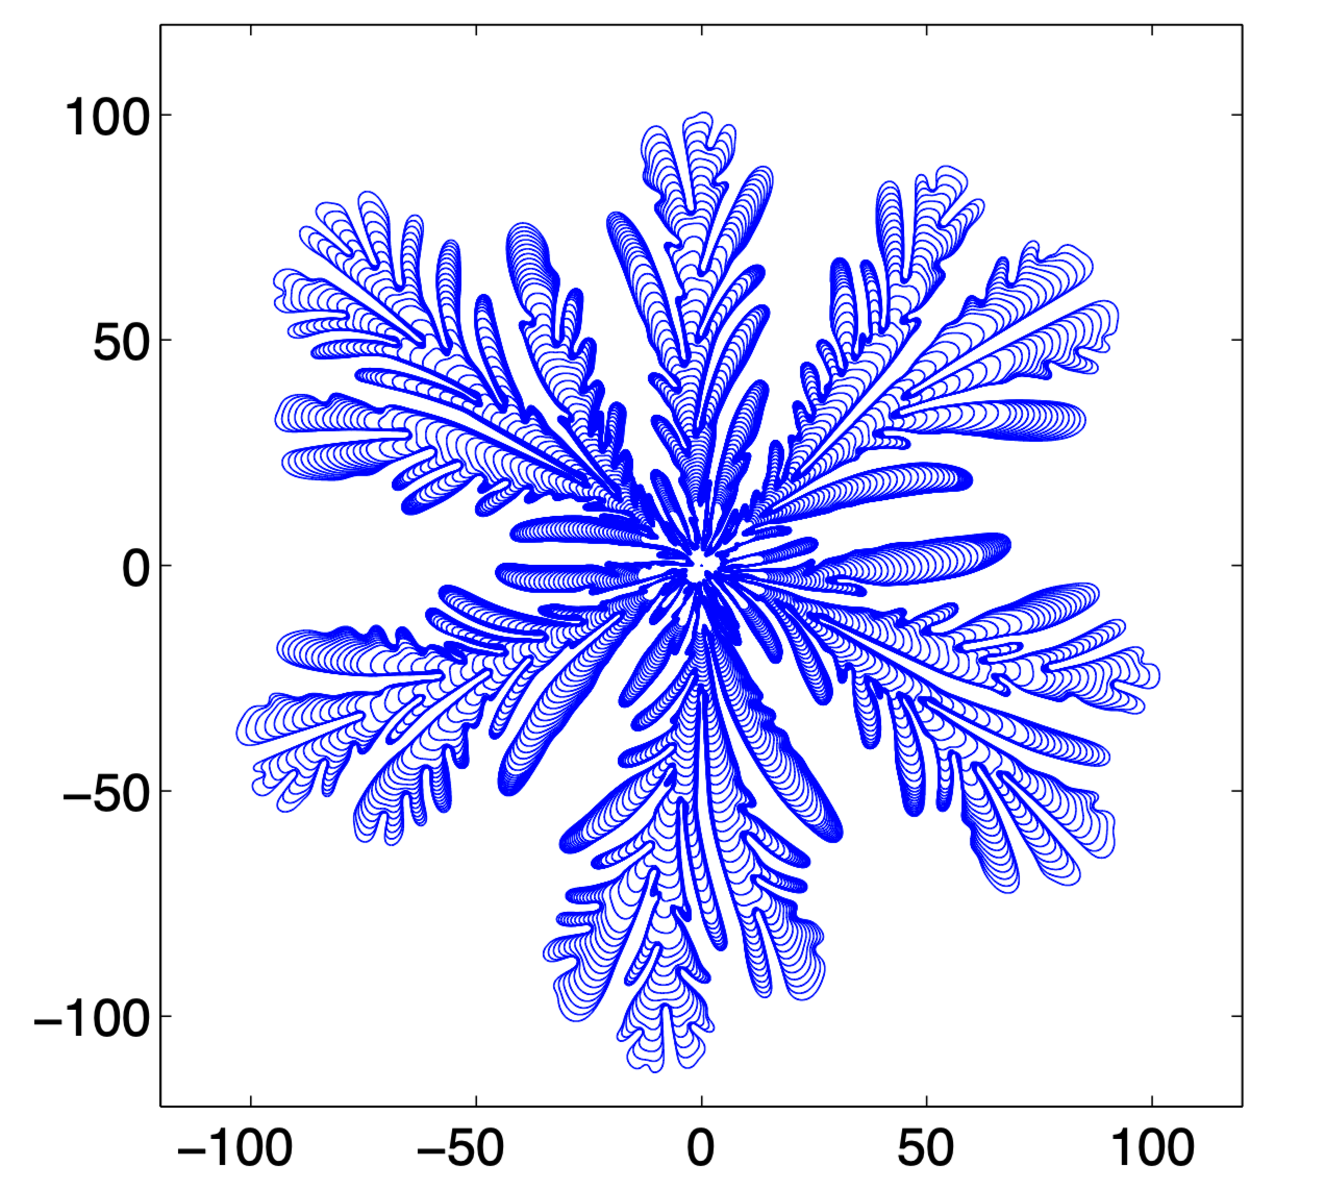
\includegraphics[scale=0.3]{Unstable}[a]
  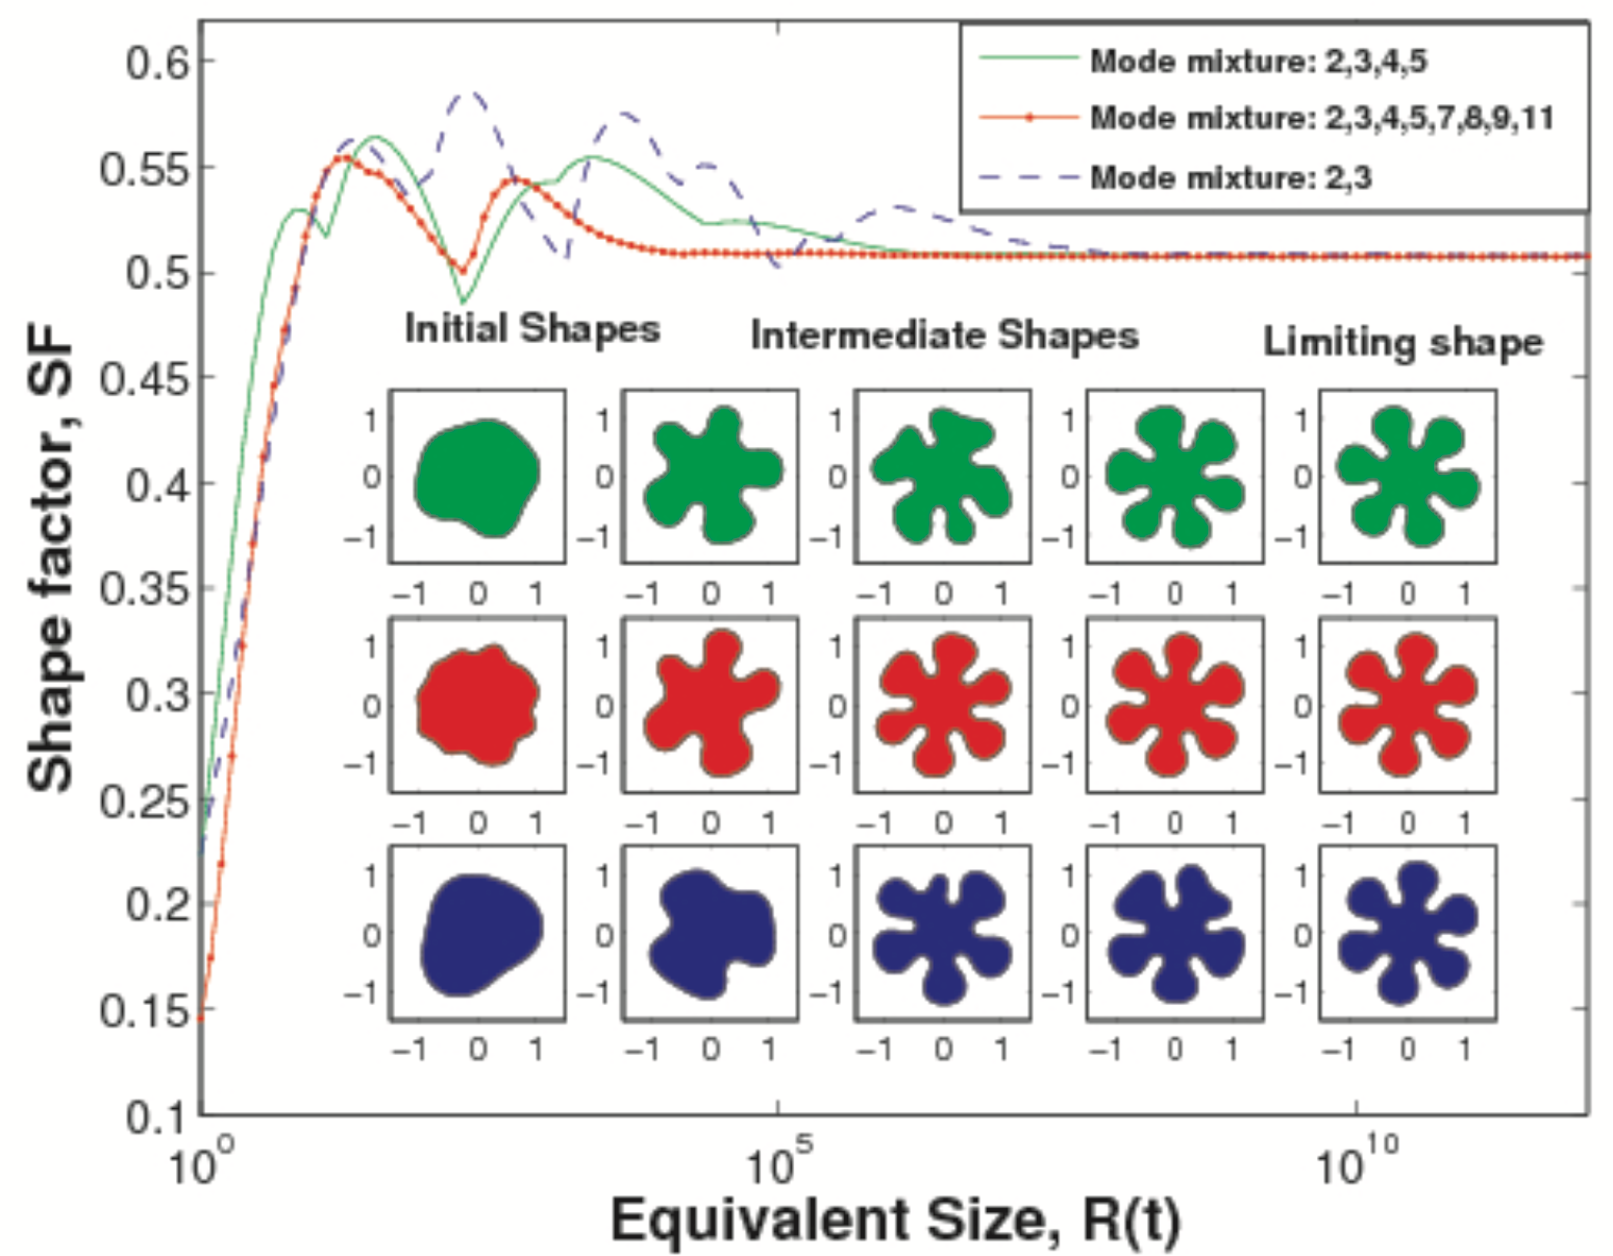
\includegraphics[scale=0.28]{Stable2}[b]
  \caption{An illustration of unstable growth [a] and stable [b] dynamical patterns with six-fold symmetry in a Hele-Shaw flow.}
  \label{figA}
  \end{figure}

There are many potential applications of this work due to the ubiquity of pattern-forming systems that are driven out of equilibrium. The interest in understanding the formation kinetics and the interplay of system parameters is to provide understanding of growth and form in nature as well as to achieve improved control and efficiency in a variety of physical, biological and engineering systems. For example, in industrial oil recovery techniques, where process strategy is to inject fluids (water, supercritical $CO_2$, surfactants, etc.) into oil containing porous media to push out the oil, the main problem is that the interface between the injected fluid and the oil becomes unstable, and fingers of injected fluid grow and advance, instead of pushing the oil out. Thus, the time-dependence of the injection rate may play an important role in process efficiency, by ameliorating or enhancing instability. Many problems in biology also involve pattern-forming systems (e.g. bacteria colonies, biofilms, etc) where the driving force (cell-proliferation, pressure, flow, etc.) and resistive forces (e.g. elastic membranes, production/destruction of extracellular matrix scaffolds) interact. We anticipate that the tools developed here may be adapted to provide insight to these problems.


The proposed sample project is expected to provide an understanding of growth and form for such problems, and our  coupled mathematical and statistical machine learning approachs also expected have application beyond the present context. Students will receive interdisciplinary training while performing the proposed work. This research project can involve undergraduates from various disciplines and provides an opportunity for students to apply and develop their teamwork spirit, project management, communication, and ethical behavior skills.
